%%% Dateikodierung: UTF-8
%%% äöüÄÖÜß  <-- keine deutschen Umlaute hier? UTF-faehigen Editor verwenden!

%%% Magic Comments zum Setzen der korrekten Parameter in kompatiblen IDEs
% !TeX encoding = utf8
% !TeX program = pdflatex 
% !TeX spellcheck = de_DE
% !BIB program = biber

\documentclass[master,english,smartquotes]{hgbthesis}
% Zulässige Optionen in [..]: 
%    Typ der Arbeit: 'diploma', 'master' (default), 'bachelor', 'internship' 
%    Hauptsprache: 'german' (default), 'english'
%    Option zur Umwandlung in typografische Anführungszeichen: 'smartquotes'
%    APA Zitierstil: 'apa'
%%%-----------------------------------------------------------------------------

\RequirePackage[utf8]{inputenc} % bei Verw. von lualatex oder xelatex entfernen!

\graphicspath{{images/}}  % Verzeichnis mit Bildern und Grafiken
\logofile{logo}           % Logo-Datei: images/logo.pdf (kein Logo: \logofile{})
\bibliography{references} % Biblatex-Literaturdatei (references.bib)

%%%-----------------------------------------------------------------------------
% Angaben für die Titelei (Titelseite, Erklärung etc.)
%%%-----------------------------------------------------------------------------

%%%\title{Peer to Peer File Sharing Netzwerke}
%%%\author{Andreas Zauner}
%%%\programname{Software Engineering}

%\programtype{Fachhochschul-Bachelorstudiengang} % auswählen/editieren
%%%\programtype{Fachhochschul-Bachelorstudiengang}

%%%\placeofstudy{Hagenberg}
%%%\dateofsubmission{2021}{07}{15} % {YYYY}{MM}{DD}

%%%\advisor{Alois B.~Treuer, Päd.\ Phil.} % optional

%\strictlicense % restriktive Lizenz anstatt Creative Commons (nicht empfohlen!)

%%%-----------------------------------------------------------------------------
\begin{document}
%%%-----------------------------------------------------------------------------

%%%-----------------------------------------------------------------------------
\frontmatter                                       % Titelei (röm. Seitenzahlen)
%%%-----------------------------------------------------------------------------
 
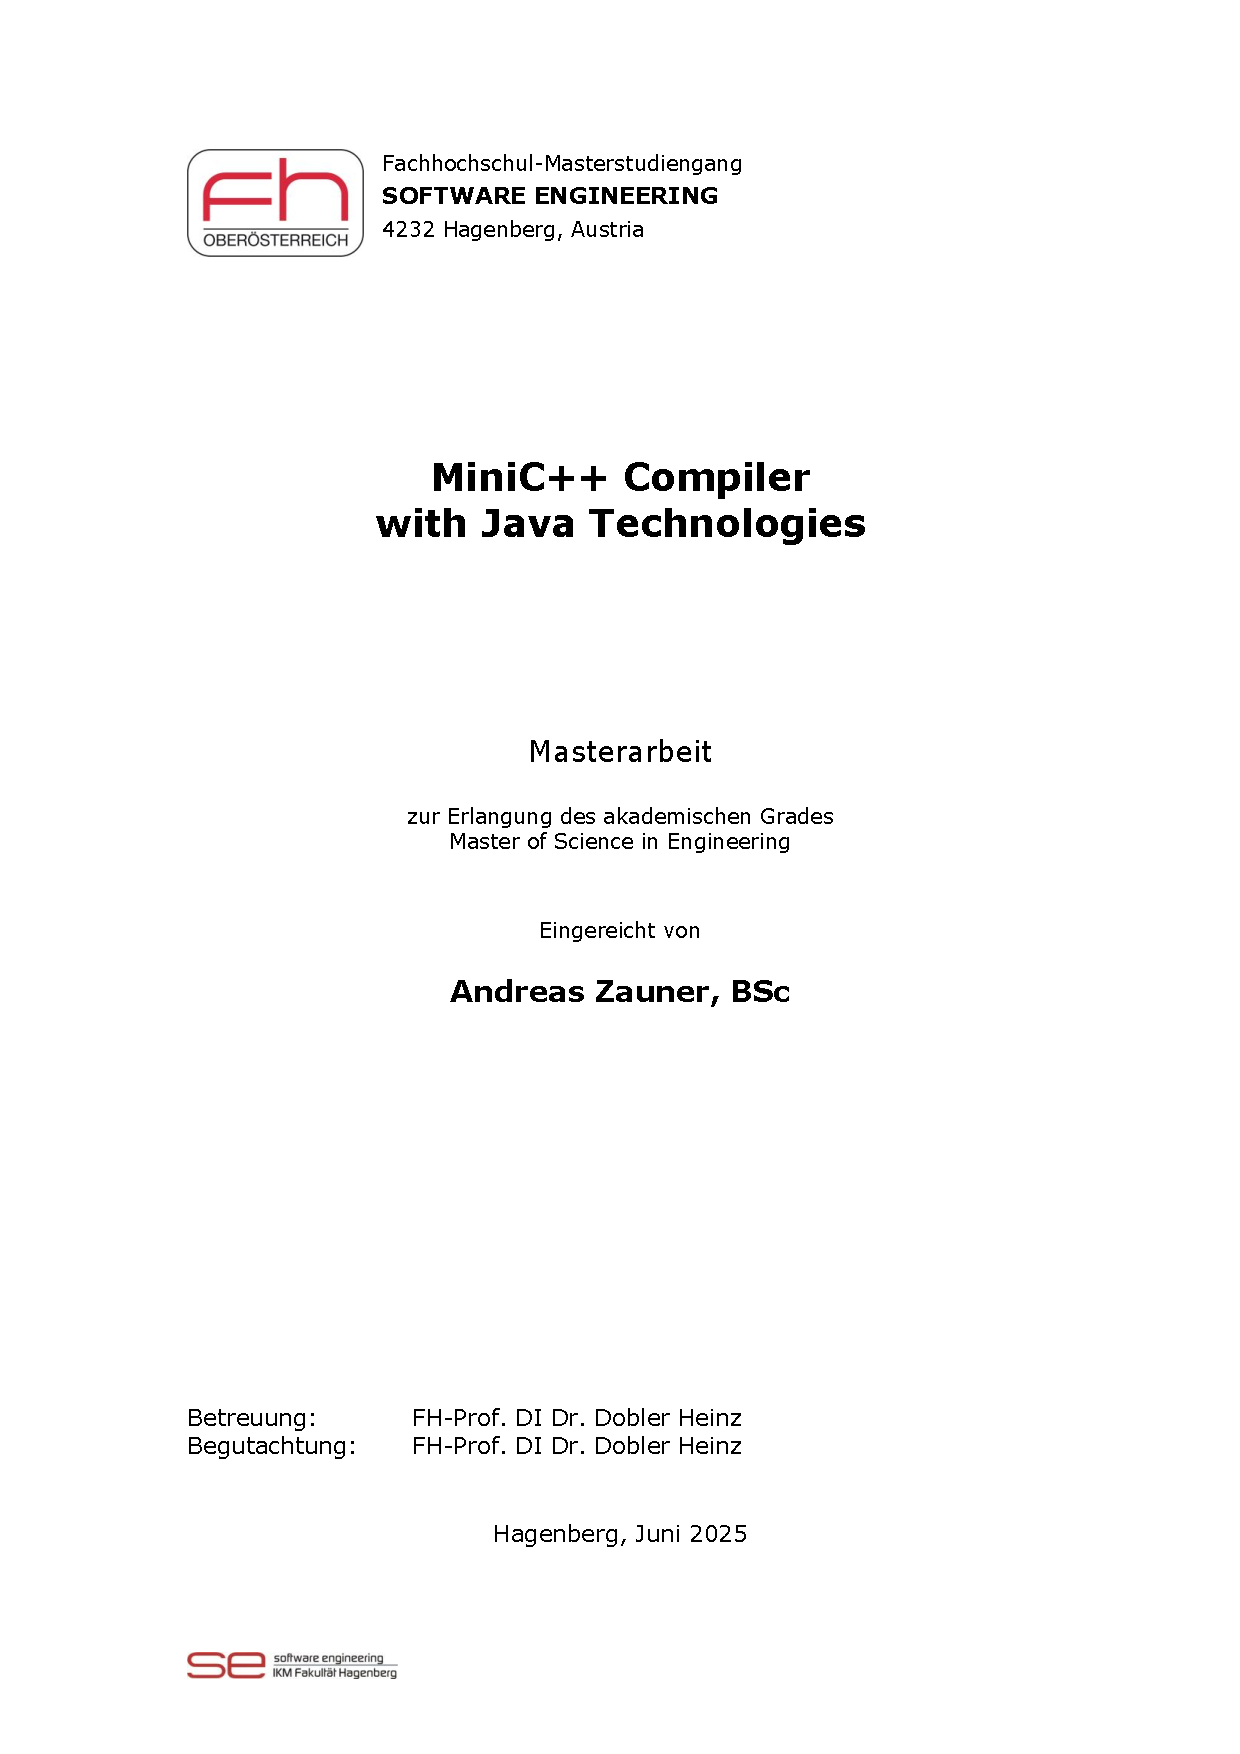
\includepdf[pages=1]{Titelblatt_Masterarbeit.pdf}
\includepdf[pages=2, pagecommand={\thispagestyle{plain}}]{Titelblatt_Masterarbeit.pdf}

\tableofcontents

\chapter{Kurzfassung}


\begin{german}

Diese Masterarbeit implementiert einen Compiler für MiniC\verb++| unter der Verwendung von Java-Technologien zur Erzeugung von Java-Bytecode. Für das Frontend wird der kombinierte Lexer- und Parsergenerator ANTLR verwendet, während das Backend die ObjectWeb ASM Bibliothek für die Bytecodegenerierung nutzt. Ähnlich zu Generatoren wie Coco-2 generiert ANTLR den Quellcode für einen Parser auf der Grundlage einer vorgegebenen Grammatik. ANTLR kann Code in mehreren Hostsprachen generieren; für diese Arbeit wurde Java gewählt. 

ANTLR ist ein Open-Source-Tool für die Spracherkennung. Es wurde erstmals 1992 veröffentlicht und wird seitdem von Terrence Parr kontinuierlich weiterentwickelt. In der aktuellen Version von ANTLR wird der adaptive-LL(*)oder ALL(*)-Parsing-Algorithmus verwendet. Dieser Algorithmus führt die Grammatikanalyse zur Parse-Zeit durch und überkommt dadurch die Einschränkungen früherer Versionen. ALL(*) erfordert nicht die Angabe einer maximalen Anzahl von Lookahead-Tokens. Stattdessen passt es sich an den aktuellen Kontext an und adaptiert die Anzahl der Lookahead-Token entsprechend.

Um einen abstrakten Syntaxbaum (AST) mit ANTLR zu erzeugen, werden drei Methoden unterstützt: Das Visitor-Pattern, das Listener-Pattern und die Verwendung einer attributierten Grammatik (ATG). Das Compiler-Frontend wird mit allen drei Methoden implementiert. Die drei Implementierungen werden in mehreren Aspekten verglichen und auf dieser Grundlage wird eine Empfehlung ausgesprochen.

ObjectWeb ASM ist eine in Java geschriebene Bibliothek zur Erzeugung von Java-Bytecode. Sie ist Open-Source und wird seit 2002 von Eric Bruneton entwickelt. Die Bibliothek wird in Compilern verwendet, die Java-Bytecode ausgeben, wie z.B. dem Kotlin-Compiler. Zur Generierung von Bytecode wird die auf dem Visitor-Pattern basierende API verwendet. 

Alle drei Frontend-Implementierungen sind mit dem Backend zu einer Anwendung verbunden, die Java-Bytecode aus MiniC\verb|++|-Code erzeugen kann. 

\end{german}
		
\chapter{Abstract}


\begin{english} %switch to English language rules
Peer-to-peer networks offer an alternative to the classic client-server model for exchanging data. In peer-to-peer networks, all clients communicate with each other. This means that the server, as the central element, can be omitted. This characteristic enables peer-to-peer networks to function even if individual participants in the network fail. In addition, peer-to-peer networks use the upload bandwidth of the individual clients, which is usually unused in traditional file sharing. 

This bachelor thesis deals in detail with peer-to-peer networks. First, known peer-to-peer networks are introduced and their characteristics are explained. Then it is shown where companies and organisations utilize peer-to-peer networks. A distinction is made between freely available networks and networks developed by companies themselves. Finally, a client for the BitTorrent network is developed. This client is able to exchange a file with other peers using the BitTorrent protocol. This shows how data exchange in a peer-to-peer network works on a technical level and which technologies are required for this.
\end{english}

			

%%%-----------------------------------------------------------------------------
\mainmatter                             % Hauptteil (ab hier arab. Seitenzahlen)
%%%-----------------------------------------------------------------------------

\chapter{Introduction}
\label{cha:introduction}

\section{Motivation}

Compilers are the backbone for computer programming. A compiler translates human-readable source code into something a computer can execute. This allows developers to focus on the functionality of the application, without having to worry about the technicalities of the concrete computer where the software will run on. For one programming language there may exist multiple compilers targeting different kinds of computers. This allows the same source code to run for example on Linux and Windows computers with Intel or ARM processors. This flexibility saves developers a lot of work, because they don't need to rewrite their application in the case they also want to target another operating system and/or processor. Furthermore, there exist compilers that target virtual machines like the Java Virtual Machine (JVM)\footnote{https://openjdk.org/groups/compiler/}. Generating code for a virtual machine has the advantage that there is no need for compilers for every target operating system and/or processor. Instead, for each operating system an implementation of the virtual machine is provided.

The process of compiling source code begins in the frontend of the compiler. The frontend reads the source code and constructs an abstract syntax tree (AST). The AST is a representation of the source code in memory. It contains only the necessary information that is needed to generate target code. The process of constructing the AST is based on the grammar of the programming language. Based on this grammar a lexer and parser are either written manually or get generated by a parser generator tool like ANTLR. In the case of ANTLR the generated lexer and parser by default construct a full parse tree from the input. From the parse tree an AST can be constructed using for example the visitor pattern. 

The AST functions then as the input for the backend of the compiler: The backend generates code for the target system. In the case of the JVM this is the so called bytecode.  APIs exist that provide an abstraction layer for the code generation. One API for bytecode generation is the open source project ObjectWeb ASM or just ASM \parencite{bruneton2007asm}. It provides an API that utilizes the visitor pattern to generate bytecode instructions. 


\section{Task and Goal}

MiniC++ is a subset of the C++ programming language. The scope of MiniC++ is very limited in comparison to C++. It is used at the University of Applied Sciences Upper Austria in Hagenberg for teaching software engineering master students about compilers in the formal languages class. In this class, all aspects of a compiler are discussed. First, the principles of lexers and parsers are explained. Then the concepts of syntax trees and further abstract syntax trees are introduced. Finally, code generation is explained. 

In the exercises, students use a MiniC++ compiler to compile MiniC++ source code to the .NET Common Intermediate Language (CIL). The frontend of the compiler is generated by using the compiler generator Coco-2 \parencite{doblerCoco2}. Which generates both, the lexer and the parser. There is only one input-file required for the definition of the lexer and the parser. Furthermore, attributes and semantic actions can be included to create an attributed grammar (ATG). 

In this master thesis, another compiler for MiniC++ will be created. This compiler will be built upon Java technologies. Output of the compiler will be Java bytecode that can be executed on the Java Virtual Machine (JVM). The frontend is based on a lexer and parser generated by the parser generator ANTLR\footnote{https://www.antlr.org/} (ANother Tool for Language Recognition). They are used to generate a full syntax tree. From this syntax tree an abstract syntax tree (AST) is constructed. The backend utilizes the ObjectWeb ASM\footnote{https://asm.ow2.io/} library. This library provides an API to generate Java bytecode. 

This master thesis will further explore the capabilities of ANTLR. ANTLR provides multiple ways to interact with the generated parser. The master thesis compares the advantages and disadvantages of each of these options.

\section{Theoretical Fundamentals}

This section explains the basic concepts of formal languages and how they are used in compilers. Furthermore, the individual components of a compiler are highlighted. 

\subsection{Formal Languages and Compilers}

Formal languages make up the fundament on which compilers are built upon. In comparison to natural languages, formal languages have a strict syntax which can be defined by a grammar. This grammar does not evolve naturally, as it does with natural languages. A formal grammar is defined by replacement rules. A replacement rule defines that a non-terminal symbol \textit{A} can be replaced by a sequence $\alpha$. The sequence may contain terminal and/or non-terminal symbols. 

Grammars can be classified according to the Chomsky hierarchy \parencite{CHOMSKY1959137}. Chomsky classifies formal languages and their grammars into four categories. Of those, the first two are relevant for compiler construction. Namely, regular grammars and context-free grammars. The four categories are differentiated by the type of rules that can be defined. The types of rules used then define which kind of automaton is needed to recognize sentences of the given language. 

\subsubsection{Regular Grammars}

Regular grammars make up the simplest group of grammars. For a grammar to be regular all rules must be in the form of $A\rightarrow a | a B$ or $S\rightarrow \epsilon$. This means that a non-terminal symbol $A$ can only be replaced by either a terminal symbol $a$ or a terminal symbol $a$ followed by a non-terminal symbol $B$. The only exception is the root rule $S$ which can be replaced by the empty sequence. 

To recognize a sentence of a regular grammar a finite automaton (FA) can be used. A deterministic FA (DFA) consists of the following elements:

\begin{itemize}
    \item $S$ finite, non-empty set of states,
    \item $\Sigma$ finite, non-empty set of symbols (alphabet),
    \item $s_0$ initial state, $s_0 \in S$,
    \item $\delta$ state transition function, $S \times \Sigma \rightarrow S$ and
    \item $F$ set of final states, $F \subseteq S$.
\end{itemize}

The DFA proceeds to read the symbols in $\Sigma$ one symbol at a time. The current symbol is then used in combination with the current state in the state transition function to acquire a new state. This process is continued until a final state is reached, meaning that a sentence has successfully been recognized. In case that for the current symbol and state no entry in the state transition function can be found, the recognition failed, and the given input is not a sentence of the language. 

A DFA can be implemented in a program to efficiently recognize sentences of a language. For more complicated regular languages nondeterministic finite automata (NFA) are easier to construct. A NFA program however is more complicated and slower compared to a DFA one. Every NFA can be transformed to a DFA to overcome this limitation. After transformation the constructed DFA may have more than the minimal number of states needed. A second transformation can be performed that reduces the DFA to a minimal DFA. 

\subsubsection{Context-Free Grammars}

Context-free grammars are the second group of grammars according to the Chomsky hierarchy. Context-free grammars include regular grammars, meaning that every regular grammar is also a context-free grammar. A replacement rule of a context-free grammar is in the form $A \rightarrow \beta$. Meaning that a non-terminal symbol $A$ can be replaced by a sequence $\beta$ containing terminal and/or non-terminal symbols or also $\varepsilon$, the empty sequence. 

In a context-free grammar central recursion is possible (direct or indirect). This allows the nested structures that are needed for programming languages, e.g., for expression hierarchies. Central recursion cannot be handled by a FA, for this a pushdown automaton (PDA) is needed. With a deterministic pushdown automaton (DPDA) all deterministic context-free grammars can be recognized. To recognize all context-free grammars a nondeterministic pushdown automaton (NPDA) is needed. For programming languages deterministic context-free grammars are used. 

There are two strategies for constructing a syntax tree from a sentence of a context-free grammar, namely top-down and bottom-up. Which strategy can be used depends on the kind of deterministic context-free grammar that is used. Following are the two most important conditions for context-free grammars:

\begin{itemize}
    \item \textbf{LL($k$) Condition:} Defines that a maximum of $k$ symbols look ahead are sufficient to deterministically decide on the next rule when using the \textit{top-down} strategy.
    \item \textbf{LR($k$) Condition:} Defines that a maximum of $k$ symbols look ahead are sufficient to deterministically decide on the next action(shift or reduce) when using the \textit{bottom-up} strategy.
\end{itemize}

The higher the value of $k$, the more complicated parsing becomes. Therefore, LL($1$) and LR($1$) grammars are preferred. For an LL($1$) or LR($1$) grammar only one symbol look ahead is needed for a deterministic decision. 

LL($k$) grammars can be recognized with a normal DPDA. For LL($1$) grammars it is also feasible to implement an efficient recursive descent parser. In the case of an LR($1$) grammar, the DPDA must be extended to be able to use an arbitrary amount of symbols on top of the stack. Only then is it able to recognize a sentence of an LR($1$) grammar with the \textit{bottom-up} strategy. It has to be noted that a DPDA which is able to recognize LR($k$) grammars, is also able to recognize LL($k$) grammars.

\subsection{Compiler Construction}

The task of a compiler is to translate code of a given source language into code of a target language. The source language being a human-readable programming language like Java and the target language being code for a given operating system and processor architecture, or a virtual machine. Compiling code can be separated into two main stages: frontend and backend.
The frontend executes of the following steps:
\begin{itemize}
    \item lexical analysis,
    \item syntactic analysis,
    \item semantic evaluation and
    \item intermediate language generation.
\end{itemize}

The backend performs optimization and code generation.

%\subsubsection{Lexical Analysis}
The lexical analysis is the first step of the compilation. It reads the source code and organizes it. The goal is to group individual characters into symbols and to skip meaningless characters (e.g., comments). The grammar of the source language provides the information about the symbols. This part of the grammar is defined using a regular grammar. 

The symbols can be divided into terminal symbols and terminal classes. Terminal symbols are special symbols like \texttt{=}, \texttt{(}, \texttt{-} and the keywords of the source language, e.g., \texttt{int}, \texttt{break},  \texttt{function}. Terminal classes are for example all numbers or identifiers. Comments are also handled at this step. Since comments usually have no influence on the generated code, they are removed. All recognized symbols are then passed to the parser (syntactic analysis and semantic evaluation). 


%\subsubsection{Syntactic Analysis}

The syntactic analysis takes the terminal symbols and classes recognized in the lexical analysis phase as input to construct the syntax tree. A context-free grammar provides the basis for the syntax tree. During the syntactic analysis the terminal symbols are grouped into syntactic elements according to the grammar. Furthermore, the syntactic integrity is also checked. In case that there is no grammar rule available for the current terminal symbol, the syntactic analysis fails, and a syntax error is reported.

%\subsubsection{Semantic Evaluation}

According to the principle of syntax-directed parsing, during the syntactic analysis the semantic evaluation is performed. This may include constructing the abstract syntax tree (AST). In the AST only the relevant information for the code generation is contained. For each rule in the grammar, there may be semantic actions associated with it, that get executed when the rule is visited. The semantic actions have access to the attributes of the rule. This information is used to generate the AST.  

%Taking the AST as a basis, the intermediate language code generation is performed. This includes for example generating the symbol table. 

Afterwards, the intermediate language code is analyzed and optimized. This may include optimizations such as inlining or loop unrolling. Depending on the use case, more aggressive optimizations can also be performed. 

Finally, the code generation unit takes the optimized code and generates the appropriate instructions for the target language. 
%\chapter{Grundlagen}
\label{cha:Grundlagen}
Dieses Kapitel bietet einen Überblick über die Grundlagen von Peer-to-Peer-Netz\-werken. Es wird dargestellt, in welche Klassen sich Peer-to-Peer-Netz\-werke einteilen lassen und anhand von welchen Kriterien diese klassifiziert werden. Weiters wird jeweils ein Vertreter dieser Klassen vorgestellt.

\section{Unterteilung von Peer-to-Peer-Netzwerken}
\textcite{pourebrahimi2005survey} teilen Peer-to-Peer-Netz\-werke in zwei Gruppen ein: Hybrid und vollkommen dezentralisiert. Die Einordnung in die Gesamtheit der verschiedenen Computersysteme ist in Abbildung \ref{fig:ComputerSystems} ersichtlich.

\begin{figure}[]
    \centering
    \includesvg[scale=0.9]{computer-systems} %{CS0031}
    \caption{Einteilung von Computer Systemen. Nachempfunden von \textcite{pourebrahimi2005survey}. }
    \label{fig:ComputerSystems}
\end{figure}

Hybride Netzwerke bestehen aus einem oder mehreren Servern, welche Metadaten verwalten. Mittels diesen wird gespeichert, welche Dateien sich aktuell im Netzwerk befinden und welche Nutzer diese besitzen. Sind in einem Netzwerk mehrere Server vorhanden, so spricht man von dezentraler Indexierung und sonst von zentraler Indexierung \parencite{pourebrahimi2005survey}.

Hingegen besitzen völlig dezentrale Netzwerke keinen einzigen Server. Alle Peers sind in ihrer Funktionalität gleichwertig. Somit stellt der Ausfall von einem oder mehreren Peers keine Gefahr für die Funktionstüchtigkeit des Netzwerkes dar \parencite{pourebrahimi2005survey}. 

Folgend werden drei Peer-to-Peer Protokolle/Netzwerke vorgestellt. 
\begin{itemize}
    \item \textbf{Gnutella:} Vollkommen dezentralisiert
    \item \textbf{Napster:} Hybrid mit zentraler Indexierung
    \item \textbf{BitTorrent:} Hybrid mit dezentraler Indexierung
\end{itemize}

\section{Gnutella}
Als Basis für den folgenden Abschnitt dient die Spezifikation des Gnutella-Protokolls \parencite{GnutellaProtocol}.

\subsection{Überblick}
Gnutella wurde im Jahr 2000 von Justin Frankel entwickelt.
Das Protokoll hat die Aufgabe, den Kontakt zwischen zwei Peers, welche Daten austauschen möchten, herzustellen. Einzelne Peers innerhalb des Gnutella-Netzwerkes werden \emph{Servents} genannt. 

\subsection{Relevanz}
Gnutella ist im Gegensatz zu anderen Protokollen, wie BitTorrent und Napster, ein völlig dezentral-organisiertes Netzwerk. Dadurch gibt es keinen einzelnen Punkt, welcher das Netzwerk zu Fall bringen könnte. Im Gnutella-Protokoll selbst ist zudem der eigentliche Datenaustausch zwischen den Servents nicht enthalten, sondern wird auf ein anderes Protokoll (siehe Kapitel \ref{sec:GnutellaAufbau}) ausgelagert.

\subsection{Aufbau}
\label{sec:GnutellaAufbau}
Das Gnutella-Protokoll bildet ein gesammeltes Netzwerk, in dem alle Servents miteinander verbunden sind. Zur Kommunikation innerhalb des Netzwerkes gibt es fünf verschiedene Nachrichtenarten:
\begin{itemize}
    \item \textbf{Ping} wird benutzt, um neue Servents im Netzwerk zu finden. 
    \item \textbf{Pong} sendet ein Servent als Antwort auf einen Ping. Die Antwort enthält die IP-Adresse des Servents und eine Angabe über die Menge an Daten, die er dem Netzwerk bereitstellt. 
    \item \textbf{Query} enthält einen Suchtext, mit welchem das Netzwerk nach Dateien abgefragt werden kann. 
    \item \textbf{Query-Hit} wird versendet, wenn ein Servent eine in einer Query angefragte Datei bei sich lokal vorhanden hat.
    \item \textbf{Push} ermöglicht es einem Servent, welcher aufgrund von Firewall-Problemen nicht selbst die Verbindung aufbauen kann, von einem anderen Servent die Verbindungsanfrage zu erhalten.
\end{itemize}
Über das Netzwerk versendete Nachrichten, werden mittels Broadcast\footnote[1]{Jeder Servent leitet die erhaltene Nachricht an alle mit ihm verbundenen Servents weiter. Ausgenommen ist hiervon der Servent, von dem die Nachricht erhalten wurde.} propagiert.
Damit einzelne Nachrichten nicht endlos lange propagiert werden, verwendet Gnutella zwei Kontrollfelder in jeder Nachricht. Das erste Feld speichert, wie viele Sprünge eine Nachricht bereits hinter sich hat. Das zweite, wie viele Sprünge noch möglich sind (Time to live, TTL). Die Auswirkungen dieser Statistiken auf die Propagation einer Nachricht sind analog zu denen in der dritten Schicht des OSI-Modells. 

Jede Nachricht enthält eine im Netzwerk eindeutige ID, mit der Antworten wieder an den Absender zurückgesendet werden können. Leitet ein Servent eine Nachricht weiter und bekommt später eine neue Nachricht, beispielsweise einen Query-Hit zurück, so kann er anhand dieser ID den Servent ermitteln, an den die Nachricht zurückgesendet werden muss.

Wird über das Protokoll ein Servent gefunden, welcher die gewünschte Datei besitzt, kann eine Verbindung mit diesem aufgebaut werden. Da der Download von Dateien nicht im Gnutella-Protokoll enthalten ist, wird dafür auf HTTP zurückgegriffen. In der Query-Hit-Nachricht sind die nötigen Informationen enhalten, damit an den Servent eine HTTP-GET-Anfrage, für die gewünschte Datei, gesendet werden kann.


\subsection{Schwächen des Protokolls}
\label{sec:GnutellaWeaknesses}
Der Mechanismus der Breitensuche zur Verteilung von Nachrichten im Gnutella-Netz\-werk generiert eine signifikante Menge an Daten. Eine Suchanfrage im Netzwerk (bei Nutzerzahlen in der Größe von Napster, siehe Kapitel \ref{sec:NapsterÜberblick}) generiert bereits 800MB an Daten. Bei durchschnittlich drei Anfragen pro Sekunde führt dies bereits zu 2.4GB/s. Anzumerken ist, dass diese Werte sich rein auf das Gnutella-Protokoll beziehen. Der eigentliche Download von Dateien ist hier nicht inkludiert  \parencite{ritter2001gnutella}.

Analysen des Gnutella-Netzwerkes zeigen, dass bereits das Entfernen von einigen wenigen Servents zu Problemen in der Konnektivität führen kann. Dadurch können sehr effektiv Denial-of-Service Attacken durchgeführt werden \parencite{ripeanu2001peer}. 

Das Netzwerk kann auch dazu benutzt werden, Distributed-Denial-of-Ser\-vice-At\-tacken gegen andere Hosts durchzuführen. Ein böswilliger Servent antwortet auf alle Query-Nachrichten mit der IP-Adresse eines Hosts, den er attackieren möchte. Der böswillige Servent gaukelt vor, die angefragte Datei zu besitzen. Nun versucht der gutmütige Servent eine Verbindung zum Opfer aufzubauen. Wenn der böswillige Servent auf genügend Anfragen antwortet, kann dadurch das Opfer in die Knie gezwungen werden \parencite{zeinalipour2002exploiting}.

\section{Napster}
\subsection{Überblick}
\label{sec:NapsterÜberblick}
Das Unternehmen Napster entwickelte ein gleichnamiges Programm zum Austauschen von Dateien. Den Fokus legte Napster vor allem auf den Austausch von Musik. So zählte Napster von seiner Veröffentlichung im Jahr 1999 bis 2001 knapp 60 Millionen Nutzer~\parencite{poblocki2001napster}. Napster sah sich jedoch mit Klagen aus der Musikindustrie konfrontiert. Nachdem Napster mehrere Klagen verlor, wurden sie gerichtlich gezwungen den Betrieb einzustellen.

\subsection{Relevanz}
Im Gegensatz zum völlig dezentral organisierten Gnutella, verfolgte Napster einen anderen Zugang zur Strukturierung eines Peer-to-Peer-Netzwerkes. Man setzte auf einen zentralen Server,
 welcher die Nutzer miteinander verknüpfte (siehe Kapitel \ref{sec:NapsterAufbau}). Somit ist Napster ein hybrides Peer-to-Peer-Netzwerk mit zentraler Indexierung. Der Erfolg von Napster führte dazu, dass andere Peer-to-Peer-Netzwerke, wie BitTorrent oder Soulseek, ihre respektiven Netzwerke in einer ähnlichen Struktur mit einem gewissen Grad an Zentralisierung aufbauten. 

\subsection{Aufbau}
\label{sec:NapsterAufbau}
Die Grundlage für den folgenden Abschnitt bildet die Spezifikation von Napster. Da keine offizielle Spezifikation verfügbar ist, wird auf eine alternative Spezifikation zurückgegriffen. Diese wird vom Entwickler des Open-Source Napster-Clients Opennap bereitgestellt \parencite{napsterSpecification}. 

Damit ein Nutzer Zugriff zum Netzwerk erhält, wird ein Account beim zentralen Napster Server benötigt. Dieser Server bildet das Herzstück des Netzwerkes. Zur Kommunikation zwischen Server und Client wird ein eigenes Protokoll auf Basis von TCP verwendet. Der Server bietet folgende Funktionen, welche für den Datenaustausch relevant sind:

\begin{itemize}
    \item \textbf{Teilen einer Datei:} Der Nutzer gibt dem Server bekannt, dass er eine oder mehrere Dateien besitzt. Diese können nun von anderen Nutzern angefordert werden. 
    \item \textbf{Downloadanfrage:} Es wird eine Anfrage an den Server gesendet, eine Datei von einem anderen Nutzer downloaden zu dürfen. Der Server antwortet mit den Informationen, welche benötigt werden, damit eine Verbindung zu dem Nutzer aufgebaut werden kann.
    \item \textbf{Datei suchen:} Per Suchtext können die Dateien, welche von anderen Nutzern geteilt werden, durchsucht werden. Es können mehrere Suchkriterien, wie beispielsweise die Bitrate, angegeben werden.
\end{itemize}
Der Napster Server bietet zusätzlich Funktionalitäten wie Chats und Freundeslisten an, jedoch sind diese für den Datenaustausch nicht wichtig.

Der reguläre Ablauf eines Datenaustausches über das Napster-Netzwerk sieht daher wie folgt aus: Ein Nutzer sendet als erstes eine Suchanfrage an den Server. Dieser antwortet mit einer Liste von Nutzern, welche eine passende Datei über das Netzwerk teilen. Im nächsten Schritt wird ein Nutzer ausgewählt, von dem die Datei heruntergeladen werden soll. Mit dem ausgewählten Nutzer wird nun eine Verbindung aufgebaut. Veranschaulicht wird dieser Ablauf in Abbildung \ref{fig:NapsterCommunications}. Hier ist anzumerken, dass je nach Firewall-Einstellungen ein anderer Nutzer die Verbindung aufbauen muss. Der Napster Server regelt, welcher Nutzer die Verbindung aufbauen muss. 

\begin{figure}[]
    \centering
    \includesvg[scale=1.2]{napster}
    \caption{Napster-Kommunikationen.}
    \label{fig:NapsterCommunications}
\end{figure}

Ist die Verbindung aufgebaut, so wird die gewünschte Datei übertragen. Dazu identifiziert sich der Nutzer, welcher die Datei erhalten möchte, mit seinem Napster-Benutzer\-namen und dem Namen der Datei. Optional kann noch ein Byte-Offset angegeben werden, falls ein bereits begonnener Download wieder aufgenommen werden soll. Als Antwort wird direkt die gewünschte Datei übertragen. Die Daten werden in sequenzieller Reihenfolge über die TCP-Verbindung übertragen. 

\subsection{Schwächen von Napster}
Als wohl größte Schwäche des Napster-Netzwerkes kann die Abhängigkeit des gesamten Netzwerkes vom zentralen Server gesehen werden. Wie \textcite{napsterCourtRuling} im Februar 2001 berichtete, wurde Napster gerichtlich gezwungen, ihren Dienst einzustellen. Damit war auf einen Schlag das gesamte Netzwerk abgeschaltet. Somit konnten Nutzer keine Daten mehr austauschen, da der Server als Vermittlungsstelle ausfiel. Da die Server-Software nicht frei verfügbar war, konnten auch keine Server von Drittparteien betrieben werden.

Das Napster-Netzwerk war rein auf die Übertragung von mp3-Dateien ausgelegt. Andere Dateiformate wurden nicht unterstützt. Somit musste für solche Dateiformate auf andere Netzwerke zurückgegriffen werden. Um gegen diese Limitierung anzukommen, wurden auch Tools wie \emph{Wrapster} entwickelt \parencite{napsterWrapster}. Wrapster erlaubte es, beliebige Dateien in eine, von Napster unterstützte mp3-Datei einzupacken. Dadurch konnte wieder das Napster-Netzwerk für den Datenaustausch benutzt werden.

\section{BitTorrent}

\subsection{Überblick}
Im Jahr 2001 veröffentlichte \textcite{BitTorrentRelease} das von ihm entwickelte BitTorrent-Protokoll und einen dazugehörigen Client. Mittlerweile werden das Protokoll und der Client vom Unternehmen Rainberry, Inc, welches von Cohen gegründet wurde, weiterentwickelt. Das BitTorrent-Protokoll ist öffentlich verfügbar, was es Entwicklern ermöglicht, selbst eigene Clients zu implementieren. \textcite{BitTorrentClientMarketshare} veröffentlichte eine Liste der am meisten verbreiteten BitTorrent-Clients. 

\subsection{Relevanz}
BitTorrent ist ähnlich strukturiert wie Napster, jedoch mit einem entscheidenden Unterschied. Bei Napster übernimmt ein einziger Server die Indexierung aller verfügbaren Dateien. BitTorrent hingegen nutzt viele verschiedene Server. Somit betreibt es dezentrale Indexierung. 
Die Relevanz von BitTorrent spiegelt sich auch in seiner Verbreitung wider. Wie aus einem Bericht des Unternehmens \textcite{BitTorrentTrafficPaloalto} hervorgeht, war BitTorrent für 3,35\% des gesamten weltweiten Datenverkehrs verantwortlich. In der Kategorie "File-Sharing" machte BitTorrent sogar mehr als die Hälfte des gesamten Datenverkehrs aus. In einem aktuelleren Bericht von \textcite{BitTorrentTrafficSandvine} beträgt der Anteil von BitTorrent am Upload-Datenverkehr 9,7\%. Damit liegt es im Ranking auf Platz Eins. 

\subsection{Aufbau}
\label{sec:BitTorrentAufbau}
Grundlage für den folgenden Abschnitt liefert die BitTorrent Protocol Specification \parencite{BitTorrentSpecification}. 
Den Kern des BitTorrent-Protokolls bildet die \emph{.torrent} Datei. Eine .torrent Datei enthält alle relevanten Metadaten, welche für den Datenaustausch
mittels des BitTorrent-Protokolls benötigt werden. Die in dieser Datei enthaltenen Metadaten bzw. die Datei selbst werden auch als „Torrent“ bezeichnet. Jeder Torrent wird anhand eines SHA1-Hashes eindeutig identifiziert. Dieser wird als \emph{Info-Hash} bezeichnet. BitTorrent ermöglicht es, neben Dateien auch ganze Ordner zu teilen. Alle Dateien und Ordner, die in einem Torrent enthalten sind, werden in sogenannte \emph{Pieces} unterteilt. Die Dateien/Ordner werden hintereinander gereiht und dann gestückelt. Jedes Piece hat die gleiche Länge, mit Ausnahme des letzten Piece, welches abgeschnitten wird. 

Ein Peer wird in zwei Kategorien unterteilt. Zum einen, die Seeder, und zum anderen, die Leecher. Als Seeder bezeichnet man einen Peer, welcher den Torrent vollständig heruntergeladen hat und diesen nun anderen zum Download zur Verfügung stellt (sogenanntes seeding). Einen Peer, der hingegen den Torrent noch nicht, oder nur teilweise, heruntergeladen hat nennt man Leecher. Dieser lädt von anderen Seeder und Leecher die Daten des Torrents herunter (sogenanntes leeching). Von einem anderen Leecher können nur die Daten, die dieser bereits heruntergeladen hat, bezogen werden. 

Die Server im BitTorrent-Netzwerk werden als \emph{Tracker} bezeichnet. Für die Verwendung dieser wird, im Gegensatz zu Napster, kein Account benötigt. Der Tracker ist ein Webserver, der Informationen zu einer Vielzahl an Torrents verwaltet. Der Tracker speichert, welche Peers aktuell einen Torrent seeden/leechen. Diese Liste wird als \emph{Swarm} bezeichnet. Der Webserver besitzt einen einzigen Endpunkt namens \emph{announce}. Möchte ein Peer beginnen, einen Torrent zu downloaden, so muss als erstes eine Anfrage an diesen Endpunkt gesendet werden. Dadurch fügt der Tracker den Peer zum Swarm hinzu. Gleichzeitig erhält der Client als Antwort vom Tracker die Verbindungsdaten von anderen Peers im selben Swarm.

Die Betreiber von Trackern bieten üblicherweise eine Website an, welche zumindest folgende Funktionalitäten bietet:
\begin{itemize}
    \item \textbf{Registrieren von Torrents:} Eine .torrent-Datei kann beim Tracker hochgeladen werden. Damit beginnt der Tracker Peers zu vermitteln. 
    \item \textbf{Suche:} Das Verzeichnis aller dem Tracker bekannten Torrents, kann durchsucht werden. Hier erhält man auch Informationen über die Anzahl der Seeder/Leecher eines Torrent. Gibt es keinen Seeder für einen Torrent so spricht man von einem "toten" Torrent.
    \item \textbf{Download einer .torrent-Datei:} Die zu einem Torrent gehörende .torrent-Datei wird zum Download angeboten. 
\end{itemize}
    
Der Austausch von Daten mit anderen Peers erfolgt über eine TCP-Verbindung. Jedoch setzt BitTorrent, im Gegensatz zu Napster und Gnutella, darauf, von mehreren Peers gleichzeitig Daten zu beziehen. Von einem Peer werden einzeln die Pieces, in denen die Daten gestückelt sind, bezogen.
Um dies zu organisieren, wird das \emph{BitTorrent-Peer-Protokoll} verwendet. 
Der BitTorrent-File-Sharing-Prozess wird in Abbildung \ref{fig:BitTorrentProcess} dargestellt.

\begin{figure}[]
    \centering
    \includesvg[width=0.75\textwidth]{bittorrent Process} %{CS0031}
    \caption{BitTorrent File-Sharing Prozess. Nachempfunden von \textcite{xia2010survey}. }
    \label{fig:BitTorrentProcess}
\end{figure}

Am Beginn einer Verbindung tauschen beide Peers einen Handshake aus. Der Peer, der die Verbindung eröffnet hat, sendet als erster seinen Handshake. Darin enthalten ist unter anderem der Info-Hash, anhand dessen der andere Peer zuordnen kann, welcher Torrent ausgetauscht werden soll. Ist der Handshake erfolgreich durchgeführt, so erfolgt die restliche Kommunikation mittels der Nachrichtenarten, die im Protokoll spezifiziert sind. Diese sind: 
\begin{itemize}
    \item \textbf{Keep-Alive} wird verwendet um zu signalisieren, dass die Verbindung noch aufrechterhalten werden soll. Wird keine Keep-Alive Nachricht (oder eine andere) innerhalb einer bestimmten Zeit erhalten, so kann die Verbindung geschlossen werden. 
    \item \textbf{Choke} teilt mit, dass man die Verbindung suspendiert. Dadurch werden keine Daten übertragen. Dies ist der Standardzustand.
    \item \textbf{Unchoke} teilt mit, dass die Verbindung nicht mehr suspendiert wird. Nun können Daten übertragen werden.
    \item \textbf{Interested} teilt mit, dass man an den Daten des anderen Peers interessiert ist.
    \item \textbf{Not Interested} teilt mit, dass man nicht an den Daten des anderen Peers interessiert ist. Dies ist der Standardzustand.
    \item \textbf{Have} informiert, dass man ein Piece heruntergeladen hat. 
    \item \textbf{Bitfield} übermittelt eine Liste an Pieces, die man bereits heruntergeladen hat. Diese Nachricht ist optional und kann nur direkt nach dem Handshake übermittelt werden. 
    \item \textbf{Request} bittet den anderen Peer um Übertragung eines Piece. Das Piece wird in \emph{Blocks} unterteilt. Für jeden Block innerhalb des Piece wird eine eigene Nachricht gesendet. Durch ein Byte-Offset wird festgelegt, welcher Block angefragt wird.
    \item \textbf{Piece} wird als Antwort auf einen Request versendet. Das Piece enthält den im Request angeforderten Block.
    \item \textbf{Cancel} teilt mit, dass man keine Antwort auf einen Request mehr benötigt. Diese Nachrichtenart wird verwendet, falls Anfragen für ein Piece an verschiedene Peers gesendet werden.
\end{itemize}

\subsection{Schwächen des Protokolls}

Die Verwendung eines BitTorrent Clients kann zu Problemen in Bezug auf die TCP-Congestion-Control führen. Zurückzuführen ist das auf die Größe der Buffer von Routern. Wie \textcite{gettys2011Bufferbloat} beschreibt, können Pakete in einem vollen Buffer mehrere Sekunden darin verweilen, bis sie versendet werden. Grundsätzlich kümmert sich die TCP-Congestion-Control darum, allen TCP-Verbindungen gleichmäßig viel Bandbreite zur Verfügung zu stellen. Da ein BitTorrent-Client aber mehrere TCP-Verbindungen aktiv betreibt, erhält der Client eine unfaire Bevorzugung. Dadurch leiden andere Applikationen im selben Netzwerk, wie beispielsweise ein VoIP-Programm, an zu hoher Latenz. Dies kann  ihre Benutzbarkeit erheblich einschränken. Das BitTorrent-Protokoll wurde aufgrund dieser Problematik erweitert. Alternativ zu TCP wurde die Möglichkeit geschaffen, eine Verbindung auch über UDP aufzubauen. \textcite{norberg2009utorrent} entwickelte dafür das \emph{uTorrent transport protocol}. Das uTorrent transport protocol setzt auf UDP auf und implementiert den Congestion-Control-Algorithmus LEDBAT (Low Extra Delay Background Transport) \parencite{shalunov2012low}. LEDBAT ermöglicht es, die maximale Bandbreite zu nutzen, wenn kein anderer Datenverkehr stattfindet. Benötigen andere Applikationen auch Bandbreite, so verringert LEDBAT seine eigene benötigte Bandbreite.
%\chapter{Vergleich Traditionell zu Peer-to-Peer}
\label{cha:Vergleich}

In diesem Kapitel erfolgt eine Gegenüberstellung von traditionellem Filesharing zu Peer-to-Peer Filesharing. Es werden die Vor- und Nachteile der jeweiligen Methoden in Bezug auf verschiedene Aspekte beschrieben.

\section{Download}
\label{sec:VergDownload}
Die Downloadgeschwindigkeit ist für Endnutzer das relevanteste Kriterium in Bezug auf einen Dateidownload. Die Geschwindigkeit, welche konkret für einen Download erreicht werden kann, ist von mehreren Faktoren abhängig. Dazu zählen:
\begin{itemize}
    \item Geschwindigkeit der Internetverbindung zum ISP.
    \item Geschwindigkeit der Internetverbindung des Content-Providers zum ISP des Endkunden.
    \item Auslastung der Internetverbindung des Content-Providers.
\end{itemize} 
Ein Content-Provider ist überlicherweise ein Unternehmen, welches Daten bereitstellt. Umso weiter der Server eines Unternehmens vom ISP des Endkunden entfernt ist, desto langsamer ist tendenziell die Verbindung. Große Unternehmen umgehen dies, indem sie auf Content-Delivery Netzwerke setzen. Dadurch ist auch ihre eigene Internetverbindung weniger belastet. Content-Delivery Netzwerke verlangen jedoch einen dementsprechenden monetären Aufwand. Dazu mehr in Kapitel \ref{sec:VergleichKosten}. 

Grundsätzlich werden hier Daten immer nur von einem einzigen Server bezogen. Folgendes Beispiel illustriert die Problematik, die auftritt, wenn mehrere Endnutzer gleichzeitig von einem Server über das Internet Daten herunterladen möchten. 

\begin{figure}[H]
    \centering
    \includesvg[width=.75\textwidth]{downloadTopology} %{CS0031}
    \caption{Beispielhafte Netzwerk Topografie.}
    \label{fig:NetworkTopography}
\end{figure}

In Abbildung \ref{fig:NetworkTopography} ist ein Netzwerk skizziert, in dem der Con\-tent-Provider eine Upload-Geschwindigkeit von 100 Mbit/s zum ISP der Endkunden hat. Angenommen der Con\-tent-Provider veröffentlicht eine große Datei (z.\,B. Videospiel) und alle Endkunden möchten diese gleichzeitig beziehen, so wird in diesem Fall die Verbindung des Con\-tent-Providers vollständig ausgelastet. Die Verbindung der Endkunden jedoch hat noch Kapazitäten frei. Dadurch dauert der Download für die Endkunden länger. Die Downloadgeschwindigkeit eines einzelnen Endkunden erhöht sich erst, wenn ein anderer den Download abgeschlossen hat. Wie \textcite{kim2007impact} zeigen, hat die Download-Geschwindigkeit einen signifikanten Einfluss auf die Zufriedenheit der Kunden. Daher kann durch langsame Download-Geschwindigkeiten mit einer Reduktion der Kundenzufriedenheit gerechnet werden. Der Content-Provider könnte dieses Problem minimieren, indem mehr in die Internetverbindung investiert wird. Das führt jedoch, unter Umständen zu nicht leistbaren Mehrkosten (siehe Kapitel \ref{sec:VergleichKosten}). 

Betrachtet man das Beispiel in Abbildung \ref{fig:NetworkTopography} erneut unter Verwendung eines Peer-to-Peer Filesharing-Netzwerkes wie BitTorrent, so verändert sich der Prozess des Datenaustausches. Möchten alle Endkunden gleichzeitig die Datei vom Content-Provider beziehen, lasten sie damit die Leitung des Content-Providers wieder vollständig aus. Jedoch erhöhen sich, im Gegensatz zu vorher, die Downloadgeschwindigkeiten der Endkunden bereits kurz nach Beginn des Downloads. Dies geschieht, da jeder Endkunde die von ihm heruntergeladenen Daten den anderen Endkunden zur Verfügung stellt. Die Endkunden können somit schneller als vorher ihren Download abschließen. 

Anzumerken ist, dass dies das Verhalten unter idealen Konditionen darstellt. Die in der Praxis mögliche Erhöhung der Downloadgeschwindigkeit hängt von den Endkunden ab. Stellten eine große Zahl der Endkunden die heruntergeladene Datei nach Vollendung des Downloads anderen Endkunden nicht weiter zur Verfügung, so müssen diese sich an den Content-Provider direkt wenden. 


\section{Kosten}
\label{sec:VergleichKosten}
 Die Kosten für den Betrieb eines Peer-to-Peer-Netzwerkes unterscheiden sich stark von den Kosten, die beispielsweise für ein Content-Delivery-Netzwerk nötig sind. Ein einzelner Server genügt, um die Funktionalität eines Peer-to-Peer Netzwerkes zu gewährleisten. Dieser Server könnte jedoch auch problemlos für traditionelle Downloads benutzt werden. Der Unterschied zu einer Peer-to-Peer basierten Lösung wird klar, sobald versucht wird, die eingesetzte Infrastruktur zu skalieren. 
 
 Der traditionelle Ansatz sieht vor, für zusätzlich benötigte Rechenkapazität/Bandbreite mehr Server zu beschaffen. Dies führt zu mehr Kosten für die Hardware und erhöht den Aufwand für die Verwaltung der Infrastruktur. Alternativ könnte auf ein Content-Delivery-Netzwerk wie Akamai oder Cloudfront zurückgegriffen werden. Um hingegen ein Peer-to-Peer-Netzwerk zu skalieren, kann, neben einer Erhöhung der Anzahl an Servern, zusätzlich auf die Endkunden als Unterstützung zurückgegriffen werden. Endkunden, welche bereits Daten heruntergeladen haben, teilen diese mit anderen Endkunden. Dadurch kann die Last auf den eigenen Servern reduziert werden. Die Einbindung der Endkunden ermöglicht die Bildung eines dezentralen Peer-to-Peer basierten Content-Delivery-Netzwerkes. \textcite{migliardi2015feasibility} entwickelten auf Basis von BitTorrent und Bitcoin eine Proof of Concept Implementierung eines Content-Delivery-Netzwerkes. Die Autoren zeigten in ihrer Arbeit, wie mittels ihres Content-Delivery-Netzwerkes kostenschonender Webauftritt für eine Gruppe von Handwerkern organisiert werden kann. 

 Ein Problem, welches auch von \textcite{migliardi2015feasibility} angesprochen wurde, ist, dass für ein ordentlich funktionierendes Content-Delivery-Netzwerk zu jeder Zeit ausreichend Rechner mit dem Netzwerk verbunden sein müssen. Ist dies nicht der Fall, so muss mit Beeinträchtigungen oder Ausfällen des Netzwerkes gerechnet werden. 

 Eine Kombination aus einem klassischen Content-Delivery-Netzwerk und einem Peer-to-Peer-Netzwerk zu einem gemeinsamen hybriden Netzwerk, stellt eine Möglichkeit dar, dieses Problem zu minimieren. \textcite{xu2006analysis} analysierten solch ein hybrides Netzwerk. Die Autoren konnten feststellen, dass ein hybrides Netzwerk die Reservierungskosten für Bandbreite innerhalb des Content-Delivery-Netzwerkes signifikant reduziert. Die Kostenreduktion findet ohne Einschränkung der Übertragungsqualität statt.

\section{Sicherheit}

Im folgenden Abschnitt werden mögliche Sicherheitsrisiken, die bei der Verwendung von Peer-to-Peer-Netzwerken auftreten können, vorgestellt. 

\subsection{Offene Ports}
Da in Peer-to-Peer-Netzwerken Verbindungen mit vielen verschiedenen Computern aufgebaut werden müssen, entstehen mögliche Sicherheitsrisiken. Für den Aufbau einer Verbindung wird ein offener Port bei zumindest einem Peer benötigt. Diesen Port müssen andere Peers benutzen, um erfolgreich eine Verbindung aufzubauen. Jedoch sind bei den in Haushalten vorhandenen Routern die zuständigen Firewalls standardmäßig so konfiguriert, dass kein Port geöffnet ist. Daher kann ohne Änderung an den Firewall-Einstellungen nur eine Verbindung mit anderen Peers aufgebaut werden, wenn man selber die Verbindung aufbaut. Ändert man dieses Verhalten, so ist man anfällig für potenzielle Attacken von außerhalb des eigenen Netzwerkes. 

Ein Angreifer kann mittels eines Port-Scanning-Tools, wie Nmap nach offenen Ports hinter einer IP-Adresse scannen. Findet der Angreifer einen offenen Port, weiß er, dass ein Computer hinter dieser IP-Adresse aktiv ist. Mit diesem Wissen könnte eine Distributed-Denial-Of-Service-Attacke gegen den Computer durchgeführt werden. Für die Attacke könnte das Gnutella-Netzwerk (siehe Kapitel \ref{sec:GnutellaWeaknesses}) missbraucht werden. Weiters zeigen \textcite{el2007bottorrent}, wie man unter Verwendung des BitTorrent-Neztwerkes Distributed-Denial-Of-Service-Attacken durchführen kann.


%Wie in Kapitel \ref{sec:GnutellaWeaknesses} beschrieben, könnte das Gnutella-Netzwerk für eine Distributed-Denial-Of-Service-Attacke missbraucht werden. Nicht nur das Gnutella-Netzwerk kann für eine solche Attacke benutzt werden. Wie \textcite{el2007bottorrent} zeigten, kann auch das BitTorrent-Netzerk, auf verschiedene Arten für eine Distributed-Denial-Of-Service-Attacke missbraucht werden.

\subsection{Böswillige Peers}
Ein böswilliger Peer innerhalb des Netzwerkes könnte Angriffe initiieren. Da gutmütige Peers im Regelfall offen sind für Verbindungen mit beliebigen anderen Peers, bereitet es Probleme, wenn ein böswilliger Peer aus dem Netzwerk verbannt werden soll. Die zur Identifikation nötigen Daten beschränken sich bei völlig dezentral organisierten Netzwerken wie Gnutella meist nur auf die IP-Adresse. Nur anhand der IP-Adresse einen Peer aus dem Netzwerk zu verbannen, ist jedoch ineffizient, da IP-Adressen leicht geändert werden können. Wird ein böswilliger Peer entdeckt, müsste dieser den anderen Peers mitgeteilt werden. Das Gnutella-Netzwerk enthält keinen Mechanismus, dies zu tun. Weiters erschwerend ist, dass gewährleistet werden müsste, dass der gemeldete Peer sich auch wirklich böswillig verhalten hat. 

\subsection{Validität der Dateien}
Die in Peer-to-Peer-Netzwerken ausgetauschten Daten stellen einen weiteren möglichen Angriffsvektor dar. Gelingt es, den Prozess des Datenaustausches zu manipulieren, kann Schadsoftware direkt auf dem Zielcomputer platziert werden. Die Netzwerke Gnutella und das ursprüngliche Napster sind beide sehr anfällig für eine solche Attacke. Eine Datei kann in den beiden Netzwerken auf vielen Rechnern verfügbar sein. Es gibt jedoch keine Möglichkeit zu prüfen, ob die Version einer Datei mit der von einem anderen Peer ident ist. Daher würde es genügen, dem Netzwerk bekannt zu geben, eine beliebte Datei zu besitzen, aber jedoch bei allen Download-Anfragen eine Schadsoftware zurückzusenden. Peers hätten keine Möglichkeit, die übertragene Datei zu validieren. In beiden Netzwerken werden Dateien nur immer von jeweils einem Peer heruntergeladen. Somit kann bereits mit einem Peer Schadsoftware vertrieben werden. 

BitTorrent hingegen verfolgt den Ansatz, von mehreren Peers Daten zu beziehen (siehe Kapitel \ref{sec:BitTorrentAufbau}). Die erhaltenen Daten werden pro Piece mittels eines Hashing-Algorithmus validiert. Somit kann ein Peer, welcher mutwillig schädliche Daten übermittelt, keinen Schaden anrichten. Diese Validierung stellt jedoch nur fest, ob die im Torrent beschriebenen Daten korrekt übertragen wurden. Erstellt ein Angreifer einen Torrent für eine Schadsoftware, bietet die Validierung mittels Hashes keinen Schutz. Damit dieser Angriff erfolgreich sein kann, muss der Angreifer den schädlichen Torrent in Umlauf bringen. Eine mögliche Strategie wäre, den Namen von beliebten Torrents zu missbrauchen. Unachtsame Nutzer könnten den schädlichen Torrent herunterladen und zu Opfern werden. Es gibt jedoch Möglichkeiten, schädliche Torrents zu identifizieren, bevor sie heruntergeladen wurden. \textcite{blackstonepredict} entwickelten ein Machine-Learning-Modell, mit dem schädliche Torrents identifiziert werden können. Dieses Modell ist imstande, bis zu 95\% der schädlichen Torrents auch als solche zu klassifizieren.

%auch bei traditionell

%file validation 
%faulty client
%open port
%ddos


\section{Updates}
Peer-to-Peer-Protokolle und die dazugehörigen Clients benötigen immer wieder Aktualisierungen. Hierbei gilt es zu beachten, dass Aktualisierungen nicht die Funktionalität eines bereits bestehenden Netzes beeinträchtigen. Zudem muss den Clients mitgeteilt werden, dass eine Aktualisierung vorhanden ist. Je nach Architektur des Netzwerkes bieten sich verschiedene Möglichkeiten an, Aktualisierungen vorzunehmen. 

In einem Netzwerk mit zentraler Indexierung, wie Napster, müssen Peers immer Kontakt mit dem zentralen Server suchen. Dieser Kontakt kann dazu benutzt werden, um Peers über eine anstehende Aktualisierung zu informieren. Somit lässt sich ein Update-Mechanismus analog zu klassischer Software, welche über das Internet vertrieben wird, implementieren. Dieser Ansatz wird beispielsweise von Napster genutzt. Da Napster sein Protokoll nicht öffentlich zugänglich machte und es somit nur einen einzigen offiziellen Client gab, konnte Napster den Client und das Protokoll in einem aktualisieren. 

Dieser Ansatz stößt jedoch an seine Grenzen, wenn ein Netzwerk nach dezentraler Indexierung aufgebaut ist. Ohne eine zentrale Instanz, welche vorgibt, dass eine Aktualisierung durchzuführen ist, lässt sich eine gleichzeitige Aktualisierung eines Netzwerkes schwer koordinieren. In einem völlig dezentral organisiertem Netzwerk ist ein solcher Ansatz aufgrund von fehlender Zentralisierung grundsätzlich nicht möglich. 

Daher nutzen Netzwerke wie BitTorrent und Gnutella einen anderen Mechanismus, um Aktualisierungen durchzuführen. Beide Protokolle erlauben es, Protokoll-Er\-weiterung\-en zu entwickeln. Beim Aufbau einer Verbindung können sich Peers darüber austauschen, welche Erweiterungen sie jeweils unterstützen. Alle Erweiterungen, die von beiden Peers unterstützt werden, können in der Kommunikation verwendet werden. Somit können Peers neue Funktionalitäten benutzen, wenn sie diese unterstützen und gleichzeitig eine Abwärtskompatibilität gewährleisteten. 

Für die Entwickler von Clients solcher Protokolle bietet dieser Mechanismus auch Vorteile. Sie können damit rechnen, dass ihr Client weiter funktioniert, auch wenn eine neue Erweiterung veröffentlicht wird. Aufgrund der Abwärtskompatibilität können nicht aktuelle Clients weiterverwendet werden, während andere Client-Hersteller bereits neue Erweiterungen unterstützen. 
%\chapter{Kommerzielle Anwendungsgebiete Peer-to-Peer}
\label{cha:Kommerziell}
In diesem Kapitel wird vorgestellt, wie verschiedene Unternehmen und Organisationen Peer-to-Peer Netzwerke kommerziell einsetzen. 

\section{Airdrop}
Airdrop ist ein von Apple entwickeltes Feature für iOS und macOS, welches es ermöglicht, Dateien zwischen Geräten, auf Basis von Peer-to-Peer,  auszutauschen. Nutzer können untereinander Daten austauschen, wenn sie in der Nähe voneinander sind. Airdrop nutzt eine Kombination aus Bluetooth und Wi-Fi für die Verbindung. 

Die Funktionsweise von Airdrop wird auf der Website von Apple beschrieben \parencite{appleAirdrop}. Möchte ein Nutzer Daten an ein anderes Apple-Gerät senden, müssen zuerst Bluetooth und Wi-Fi aktiviert werden. Das Gerät sendet daraufhin mittels Bluetooth-Low-Energy eine Nachricht aus. Diese Nachricht enthält Identifikationsdaten des Senders. Sind Apple-Geräte in der Reichweite des Bluetooth-Signals aktiv und haben Airdrop aktiviert, so erhalten die Geräte die Nachricht über den versuchten Verbindungsaufbau. Akzeptieren ein oder mehrere Geräte die Anfrage, wird eine Peer-to-Peer-Verbindung mittels Wi-Fi aufgebaut. Die Grundlage für die Kommunikation mittels Wi-Fi, bildet das Apple Wireless Direct Link Protocol \parencite{stute2018one}. Die Daten werden dann über die geöffnete Wi-Fi-Verbindung übertragen. Die Geräte benötigen für die Verwendung von Airdrop keine Internet-Verbindung. Die gesamte Kommunikation erfolgt lokal über die Peer-to-Peer-Wi-Fi-Verbindung. 
Airdrop ist eine proprietäre Technologie von Apple, jedoch gibt es auch Airdrop-kompatible Open-Source-Implementierungen, wie das von \textcite{openDrop} entwickelte OpenDrop. 

\section{BitTorrent}

Mehrere Unternehmen und Organisationen verwenden die BitTorrent-Technologie. Mittels der BitTorrent-Technologie stellen diese Unternehmen Daten für die Öffentlichkeit bereit, oder übermitteln diese an ihre Kunden. Folgend werden einige dieser Unternehmen und Organisationen vorgestellt. Zusätzlich wird angeführt, welche Vorteile die Unternehmen und Organisationen sich durch die Verwendung der BitTorrent-Technologie erhoffen.

\subsection{Wargaming}

Wargaming ist ein Videospielehersteller, der unter anderem mehrere Massen-Mehr\-spieler-Onl\-ine-Spiele entwickelt und betreibt. Diese sind World of Tanks, World of Warships und World of Warplanes. Laut \textcite{wotPlayerStatistics} haben sich mehr als 160 Millionen Spieler alleine für World Of Tanks registriert. 

Alle drei Spiele können über das von Wargaming entwickelte Wargaming.net Game Center heruntergeladen werden. Für die Installation von World of Tanks würden bis zu 100 Gigabyte an Speicherplatz benötigt werden. Anzumerken ist hierbei, dass die für die Installation benötigten Daten in komprimierter Form übertragen werden. Dadurch ist die Menge an Daten, die übertragen werden, etwas geringer als die vollen 100 Gigabyte. Die Größe der für das Spiel benötigten Dateien, kombiniert mit der Anzahl an Spielern, sorgt für einen erheblichen Datenverkehr. Für die Übertragung dieser Daten, verwendet das Wargaming Game Center ausschließlich BitTorrent \parencite{wargamingNetworkInteraction}. Als Vorteil führt Wargaming an, dass durch die Verwendung von BitTorrent Daten nicht nur von einem Rechenzentrum heruntergeladen werden können, sondern zusätzlich noch von Computern in der Nähe oder im lokalen Netzwerk \parencite{wargamingNetworkInteraction}. Bevor Wargaming  das Game Center verwendete, konnten die Spiele auch mittels eines beliebigen BitTorrent-Client aktualisiert werden \parencite{wotFaq}. 

Im Wargaming Game Center kann eine Maximale-Upload-Geschwindigkeit gesetzt werden oder der Upload als Ganzes unterbunden werden. Diese Einstellungen sind für Spieler mit limitierter Upload-Bandbreite relevant. Würde die gesamte Upload-Bandbreite benutzt werden, um Daten mit anderen Spielern zu teilen, wäre wenig oder keine Upload-Bandbreite mehr verfügbar, um mit dem Spielserver zu kommunizieren. Dies könnte zu hohen Latenzzeiten führen und daraus folgend die Spielqualität erheblich beinträchtigen.


\subsection{OpenStreetMap}

Mittels des OpenStreetMap Projektes kann frei auf weltweite Karten zugegriffen werden. Das Projekt sammelt Geo-Daten und macht diese frei zum Download verfügbar. Unterstützt wird OpenStreetMap durch die OpenStreetMap-Foundation. Auf ihrer Website können die Daten in Form von Karten angesehen werden. Zusätzlich können noch Routen von A nach B berechnet werden. Die von OpenStreetMap bereitgestellten Daten werden unter anderem von \textcite{osmApple} und Facebook verwendet \parencite{osmFacebook}. 

Die von OpenStreetMap gesammelten Geo-Daten haben eine Größe von aktuell 121 Gigabyte \parencite{osmPlanet}. OpenStreetMap veröffentlicht wöchentlich eine neue Version ihrer Daten. Diese können, in Form einer XML-Datei, heruntergeladen werden. Durchschnittlich werden täglich vier Millionen Änderungen an den Geo-Daten durchgeführt \parencite{osmStats}. Neben der Gesamtversion der Daten stehen auch die wöchentlichen Änderungen separat zum Download zur Verfügung. Diese umfassen circa fünf Gigabyte an Daten. 

Die OpenStreetMap-Foundation verwaltet die für den Download und Betrieb notwendigen Server. Server-Kapazitäten werden unter anderem vom University College London bereitgestellt \parencite{osmHardware}. Aus dem Finanz-Be\-richt der OpenStreet\-Map-Foundation geht hervor, dass der Großteil der verfügbaren Gelder für Hardware ausgegeben wird \parencite{osmFinances}. Finanziert wird die Open\-Street\-Map-Foun\-dation hauptsächlich von Spenden und Mitgliedsbeiträgen, wie im Finanz-Be\-richt erwähnt wird. Daher erhöhen sich mit steigenden Nutzerzahlen nicht zwanghaft die für den Betrieb der Server notwendigen Einnahmen. Bemerkbar macht sich dies auf der Download-Seite für die Geo-Daten. Aufgrund von limitierter Upload-Bandbreite, müssen Downloads auf maximal 4096 Kilobyte pro Sekunde gekappt werden \parencite{osmPlanetWarning}. 

Als Alternative zu den Direkt-Downloads wird auf Torrent-Versionen der selben Dateien verwiesen. \textcite{osmPlanetTorrent} begann 2020 mit der Verwendung von Torrents als zusätzliche Downloadmöglichkeit. Für jede neue Version der Geo-Daten wird seither ein Torrent angeboten. OpenStreetMap nennt mehrere Gründe für die Einführung von Torrents. Ist der Download-Server, wie in der vorher erwähnten Situation, überlastet, können Torrents dazu beitragen, die Server zu entlasten. Downloaden in weiterer Folge mehrere Nutzer die Geo-Daten mittels Torrents, kann ihnen dies im Vergleich zu Direkt-Downloads höhere Download-Geschwindigkeiten ermöglichen (siehe Kapitel \ref{sec:VergDownload}). 


\subsection{Linux-Distributionen}
 
Mehrere bekannte Linux-Distributionen bieten den Download ihrer Installationsdateien auch mittels Torrents an. Dazu zählen, unter anderem, \textcite{debianTorrent}, \textcite{ubuntuTorrent} und \textcite{centOSTorrent}. \textcite{debianTorrent} beschreibt auf ihrer Website, dass Downloads unter Verwendung von BitTorrent ihre Server nur minimal belasten. Durch die Verteilung der Last und das Hochladen von Daten von allen Peers können zusätzlich schnelle Downloadgeschwindigkeiten ermöglicht werden. 


\section{Windows}

Microsoft ermöglicht für sein Betriebssystem Windows und darauf aufbauender Software, Aktualisierungen auf Basis von Peer-to-Peer \parencite{microsoftP2P}. Microsoft stellt dafür zwei Methoden zur Verfügung: Delivery Optimization und BranchCache. Diese Methoden können in verschiedenen Bereichen angewendet werden. Diese sind:
\begin{itemize}
    \item \textbf{Windows Update} ermöglicht Aktualisierungen von Windows für einen Endkunden.
    \item \textbf{Windows Update for Business} ermöglicht kommerziellen Kunden zu verwalten, wann und welche Windows-Updates installiert werden. Endgeräte verbinden sich hier mit Microsoft direkt. Windows Update for Business ist eine modernere Alternative zu WSUS \parencite{microsoftWUFB}.
    \item \textbf{WSUS (Windows Server Update Services)} ermöglicht kommerziellen Kunden zu verwalten, wann und welche Windows-Updates installiert werden. WSUS wird auf einem Windows Server installiert und dient als lokale Speicherinstanz für Windows Updates innerhalb eines Netzwerkes. Geräte im Netzwerk verbinden sich mit WSUS, um Updates zu erhalten \parencite{microsoftWSUS}. 
    \item \textbf{Configuration Manager} ist eine Management-Software für die Verwaltung von Hardware und Software in einem Unternehmen. Configuration Manager kann benutzt werden, um  Aktualisierungen von Applikations-Software oder Betriebssystemen zu automatisieren \parencite{microsoftConfigMgr}. 
\end{itemize}
BranchCache besitzt im Vergleich zu Delivery Optimization beschränkte Anwendungsgebiete. Diese sind in der Tabelle \ref{tab:windowsUpdateArea} ersichtlich. Folgend wird nun näher auf die beiden Methoden eingegangen. \noindent
\begin{table}[]
    \caption{Anwendungsgebiete der Windows Peer-to-Peer-Update-Methoden. Übernommen von \textcite{microsoftP2P}. }
    \label{tab:windowsUpdateArea}    
    \begin{tabularx}{\textwidth}{L|*{4}{L} @{}} 
    \hline
    \textbf{Methode}    & \textbf{Windows Update} & \textbf{Windows Update for Business} & \textbf{WSUS}  & \textbf{Configura\-tion Manager} \\  \hline
    Delivery Optimization  & Ja                      & Ja                                   & Ja            & Ja                             \\
    BranchCache         & Nein                    & Nein                                 & Ja            & Ja              \\  \hline        
    \end{tabularx}
\end{table}

\subsection{Delivery Optimization}
Grundlage für diesen Abschnitt ist die Dokumentation von \textcite{microsoftDeliveryOpt} zu Delivery Optimization. Delivery Optimization ist eine Technologie, mit der Daten für beispielsweise Aktualisierungen von mehreren alternativen Quellen zusätzlich zu klassischen Servern bezogen werden können. Alternative Quellen sind andere Geräte innerhalb des selben Netzwerkes. Verwaltet wird Delivery Optimization in der Cloud. Daher wird für die Verwendung eine Internetverbindung und im Speziellen eine Verbindung zum Delivery Optimization Cloud Service benötigt. 
Mit Delivery Optimization können neben Windows Updates noch andere Arten von Inhalt übertragen werden. Unterstützt werden unter anderem noch Windows 10 (Business) Store Dateien, Windows Defender Updates und Microsoft Edge Browser Updates. 

Das Beziehen von Daten unter der Nutzung von Delivery Optimization kann wie folgt beschrieben werden: Basis hierfür ist die Dokumentation von \textcite{microsoftDeliveryOptWorkflow}. Am Beginn eines Downloads holt sich der Client Metadaten vom Delivery Optimization Service in der Cloud. Die Metadaten beinhalten eine Menge an SHA-256 Hashes, welche die  herunterzuladenden Daten beschreiben. Jeder Hash ist eine Prüfsumme für einen Block der Daten. Ein Block ist im Regelfall ein Megabyte groß. Die Authentizität der Metadaten wird zusätzlich noch mit einem Hash überprüft. Als nächstes baut der Client eine Verbindung mit einem sogenannten Peer Matching Service von Microsoft auf. Dieser liefert dem Client eine Liste an Peers, welche die gewünschten Daten besitzen. Der Client baut darauf hin Verbindungen mit den Peers auf. Sobald ein Block von einem Peer heruntergeladen wurde, wird dessen Hash mit dem aus den Metadaten verglichen. Fällt diese Überprüfung negativ aus, so wird der Bock verworfen. Liefert ein Peer mehrmals ungültige Blöcke, so wird dieser vom Client blockiert. Sind alle Blöcke heruntergeladen, fügt Delivery Optimization die Blöcke in eine Datei zusammen. Abschließend verifiziert der Dienst, welcher Delivery Optimization benutzt (z.\,B. Windows Update), die gesamte Datei.   

\subsection{BranchCache}

Als Grundlage für diesen Abschnitt dient die Dokumentation von \textcite{microsoftBranchCache} für BranchCache. Ziel von BranchCache ist es, für auf mehrere Standorte verteilte Unternehmen die Nutzung der WAN-Schnittstellen zwischen den Standorten zu verringern. BranchCache ist als Caching-Lösung konzipiert. Es gibt zwei Möglichkeiten, diesen Cache zu verwenden. Im Hosted Cache Modus ist an jedem Standort ein Windows Server vorhanden, welcher die Caching Aufgaben übernimmt. Im Distributed Cache Modus werden die Daten auf den einzelnen Rechnern zwischengespeichert. Bei beiden Modi ist ein zentraler BranchCache Server am Hauptstandort notwendig. Microsoft hat für BranchCache die Protokolle HTTP, SMB und BITS erweitert. Zusätzlich wurden mehrere Protokolle für die verschiedenen Kommunikationsarten von BranchCache entwickelt. Folgend wird dargestellt, wie der Austausch von Daten unter Nutzung von BranchCache abläuft. 

\subsubsection{Distributed Cache Modus}

Wenn ein Client eine Datei benötigt, sendet er im Distributed Cache Modus eine Anfrage an den zentralen Branch\-Cache-Server. Der Client teilt dem Server  in der Anfrage mit, dass er BranchCache benutzen möchte. Der Server liefert daraufhin dem Client Metadaten, welche die gewünschte Datei beschreiben. Unter Nutzung des BranchCache-Discovery-Protokolls sucht der Client nach einer Kopie der Datei im lokalen Netzwerk. Ist keine Kopie vorhanden, wendet sich der Client erneut an den Server. Dieses Mal ohne Verwendung von BranchCache. Daher übermittelt der Server nun die gewünschte Datei. Diese Datei fügt der Client nach dem Download zu seinem lokalen Cache hinzu. Benötigt ein anderer Client  die selbe Datei, kann diese nun aus dem lokalen Netzwerk bezogen werden. Es folgt wieder der gleiche Ablauf wie beim ersten Client. Jedoch meldet sich nun der Client, welcher die Datei besitzt, auf die Anfrage zurück. Mittels des BranchCache Retrieval Protocol wird die Datei übermittelt. Abschließend überprüft der Client die Authentizität der erhaltenen Datei. Dazu werden die Metadaten, welche vom Server gesendet wurden, verwendet.

\subsubsection{Hosted Cache Modus}

Die Kommunikation im Hosted Cache Modus funktioniert zu Beginn gleich wie im Distributed Cache Modus. Der Client sendet wieder eine Anfrage an den zentralen BranchCache-Server und dieser antwortet mit den Metadaten. Im Gegensatz zum Distributed Cache Modus wendet sich der Client nun an den lokalen BranchCache-Server. Dieser teilt dem Client mit, ob die gewünschte Datei im Cache vorhanden ist. Ist dies nicht der Fall, bezieht der Client die Daten vom zentralen Server. Der Download funktioniert ident wie im Distributed Cache Modus. Nachdem der Download abgeschlossen wurde, teilt der Client dies dem lokalen BranchCache-Server unter Verwendung des BranchCache Hosted Cache Protocol mit. Der Server speichert daraufhin eine Kopie der Datei. Benötigt ein anderer Client nun die selbe Datei, antwortet der lokale BranchCache-Server, dass die Datei vorhanden ist. Daher wird die Datei nicht vom zentralen Server bezogen.
%\include{chapters/lösungsdesign}
%\chapter{Implementierung}
\label{cha:Implementierung}

In diesem Kapitel wird die Implementierung des BitTorrent-Clients vorgestellt. Dazu wird zuerst auf den Aufbau der Implementierung eingegangen. Folgend wird die Implementierung der einzelnen Bestandteile näher erläutert. 

\section{Aufbau}

Der Aufbau der Implementierung ist in Abbildung \ref{fig:KlassenClient} ersichtlich. Die Abbildung zeigt die relevanten Klassen und deren Verhältnisse zueinander. Die zentrale Klasse ist hierbei der \emph{TorrentLoader}. Diese Klasse stellt die im Lösungsdesign beschriebene zentrale Einheit dar. Die \emph{TorrentLoader}-Klasse ist dafür zuständig, den Download des Torrents zu verwalten. Die einzelnen Komponenten, welche der \emph{TorrentLoader} benutzt, werden in den folgenden Abschnitten näher erläutert.  

\begin{figure}[]
    \centering
    \includesvg[width=\textwidth]{bittorrentClientKlassen} %{CS0031}
    \caption{Relevante Klassen des BitTorrent-Clients.}
    \label{fig:KlassenClient}
\end{figure}

\section{Bencode-Parser}

Die erste Komponente der Implementierung bildet der \emph{BencodeParser}. Dieser erfüllt die Aufgabe, eine beliebige Datei im Bencode-Format einzulesen und zu verarbeiten. Die Datei wird vom Parser soweit aufbereitet, dass jedes Element in einem Objekt zur Verfügung steht. Der \emph{ParsedDataExtractor} organisiert diese Objekte danach in Klassen, welche beispielsweise alle Metadaten enthalten. Da Elemente in Bencode beliebig tief verschachtelt werden können, ist der Parser auf rekursive Weise implementiert. Dies ermöglicht es, mit relativ wenig Code einen vollständigen Parser zu erstellen. Rekursiv bedeutet das, für (assoziative) Listen, welche verschachtelte Elemente beinhalten können, nochmals die selbe Parse-Methode aufgerufen wird, mit der die Liste selber geparst wurde.

In Programm \ref{prog:Parser} ist die Wurzel-Parse-Funktion ersichtlich. \emph{parseElement} sorgt dafür, dass an der aktuellen Stelle des Parse-Prozesses die korrekte spezifische Parse-Funktion aufgerufen wird. \verb|'e'| liefert keinen Wert, da dies das Zeichen ist, welches das Ende eines Elements signalisiert. \verb|parseList| und \verb|parseDictionary| rufen in ihren jeweiligen Funktionsrümpfen wieder die \verb|parseElement|-Funktion auf und sorgen somit für die Rekursion. 

\begin{program}
    \begin{GenericCode}[numbers=none]
private fun parseElement(): ParsedData? {
    return when (getCurr()) { //Zeichen an aktuelle Stelle im Parse-Prozess
        'i' -> parseInt()
        'l' -> parseList()
        'd' -> parseDictionary()
        'e' -> null
        else -> parseString()
    }
}
    \end{GenericCode}
    \caption{Parse-Funktion des Bencode-Parsers.}
    \label{prog:Parser}
    \end{program}

\section{Tracker-Kommunikation}

Die \emph{TrackerService}-Klasse sorgt für die Verbindung zwischen dem \emph{TorrentLoader} und der \emph{TrackerAPI}. Sie erhält vom \emph{TorrentLoader} die nötigen Informationen, um eine Anfrage an den Tracker zu senden. Die von der \emph{TrackerAPI} erhaltene Antwort wird unter Verwendung des \emph{BencodeParser} und \emph{ParsedDataExtractor} aufbereitet und wieder an den \emph{TorrentLoader} zurückgeliefert. 

Beim Senden einer Anfrage an den Tracker, muss auf die korrekte Encodierung der Query-Parameter geachtet werden. Dies betrifft den Info-Hash und die Peer-Id. Üblicherweise wird der Info-Hash auf den Websiten der Tracker im Hex-Format angegeben. Für die Anfrage an den Tracker wird jedoch das ISO 8859-1-Format benötigt. Zusätzlich muss der Info-Hash mittels URL-Encodierung encodiert werden.

\section{Datenaustausch}

Im folgenden Abschnitt wird die Implementierung des Datenaustausches mit einem Peer in verschiedenen Aspekten dargestellt. Dabei wird darauf eingegangen, wie der Verbindungsaufbau abläuft und darauffolgend Nachrichten ausgetauscht werden.

\subsection{Verbindungsaufbau}

Unter Verwendung der Sockets aus der Ktor-Bibliothek baut die \emph{PeerHandler}-Klasse eine Verbindung mit dem ihr zugewiesenen Peer auf. Hier wird darauf geachtet, dass der Verbindungsaufbau asynchron funktioniert und somit die anderen Verbindungen nicht blockiert werden. Ist die Verbindung aufgebaut, wird weiters der Empfang und Versand von Nachrichten in eigene Coroutines der Kotilnx.Coroutines-Bibliothek ausgelagert. Dadurch blockiert das Warten auf eine neue Nachricht nicht den Versand und umgekehrt. 

\subsection{Nachrichtenerhalt}

Werden über die Verbindung Daten erhalten, muss zuerst festgestellt werden, um welche Nachricht es sich handelt. Die ersten vier Bytes, die empfangen werden, repräsentieren die Länge der Nachricht. Das folgende fünfte Byte gibt die Nachrichten-ID an. Anhand dieser entscheidet der Client, wie die folgenden Bytes interpretiert werden müssen. Die weitere Bearbeitung findet für jeden Nachrichtentyp in einer eigenen Funktion statt. Nachdem die Nachricht behandelt wurde, wird wieder auf die nächste Nachricht in gleicher Weise gewartet. 

\subsection{Nachrichtenerstellung}

Bevor eine Nachricht versendet werden kann, wird sie zuerst von der \emph{MessageCreator}-Klasse erstellt. Diese Klasse enthält Funktionen, mit denen Nachrichten für alle im BitTorrent-Protokoll enthaltenen Nachrichtentypen erstellt werden können. Ausgenommen hiervon sind Nachrichten bezüglich Suspendierung und Interesse eines Peers. Diese Nachrichten haben immer den gleichen Aufbau und können somit fest codiert werden.

Die Nachrichten werden direkt als Byte-Arrays zurückgeliefert, wie in Programm \ref{prog:MessageCreate} ersichtlich ist. Dadurch muss sich der \emph{PeerHandler} nur noch um das Versenden kümmern. Wie im Programm ersichtlich ist, wird zuerst festgelegt, wie lange die Nachricht ist und welche ID sie besitzt. Auch bei den anderen Nachrichten im \emph{MessageCreator} ist dieser Schritt gleich. Danach folgt der nachrichtenspezifische Inhalt. Im Falle der \emph{have}-Nachricht des dargestellten Programms, bedeutet dies, den Index des Piece zu übermitteln. Für Nachrichten mit variabler Länge (z.\,B. \emph{piece}) müssen die ersten vier Byte, welche die Länge der Nachricht repräsentieren, dementsprechend angepasst werden. 

\begin{program}
    \begin{GenericCode}[numbers=none]
fun getHavePieceMessage(pieceIndex: Int): ByteArray {
    val length = 5.toByteArray() //Länge der Nachricht als ByteArray(Länge=4)
    val id = byteArrayOf(4)      //Id der Nachricht (4) als ByteArray(Länge=1)
    return length+ id + pieceIndex.toByteArray() //Kombination der Arrays
}
    \end{GenericCode}
    \caption{Erstellung der \emph{piece}-Nachricht im \emph{MessageCreator}.}
    \label{prog:MessageCreate}
    \end{program}


\subsection{Nachrichtenversand}

Nachrichten werden über die beim Verbindungsaufbau erstellte Coroutine an den Peer gesendet. Die im \emph{MessageCreator} erstellten Byte-Arrays müssen somit nur noch an den Socket übergeben werden.
Speziell für die \emph{request}-Nachricht wurden Optimierungen implementiert. Diese sollen dabei helfen, höhere Downloadgeschwindigkeiten zu erreichen. Dazu versendet der Client mehrere \emph{request}-Nachrichten für verschiedene Blöcke des Piece gleichzeitig. Dadurch muss der Client nicht für jeden Block auf die dazugehörige \emph{piece}-Nachricht warten. Der Client versucht eine gewisse Menge (in diesem Fall 10) an ausstehenden Anfragen beim Peer aufrecht zu halten. Wird eine \emph{piece}-Nachricht erhalten, versendet der Client die nächste \emph{request}-Nachricht.

\section{Dateizugriff}

Für das Speichern eines Piece und das Auslesen eines bereits vorhandenen Piece, muss regelmäßig mit der Zieldatei interagiert werden. Für kleine Dateien wäre es möglich, die gesamte Datei ins Programm zu laden, jedoch ist dies für größere Dateien nicht möglich. Daher liest/schreibt der Client nur an die Stellen in der Datei, welche vom jeweiligen Piece abhängen. Java bietet für diesen Anwendungsfall die Klasse \verb|RandomAccessFile| an. In Programm \ref{prog:FileRead} ist zu sehen, wie unter Verwendung dieser Klasse ein Block ausgelesen wird. Dabei ist der Ablauf für das Lesen und Schreiben gleich. Als erstes wird an die Position navigiert, wo mit der Datei interagiert werden soll. Danach wird eine beliebige Anzahl an Byte von dieser Position weg gelesen/geschrieben.




\begin{program}
    \begin{GenericCode}[numbers=none]
fun readBytes(pieceIndex: Int, offset: Int, length: Int): ByteArray {
    val piecePosition = pieceIndex*metainfo.torrentInfo.pieceLength+offset
    file.seek(piecePosition)      //Gehe zu Position des Piece in Datei
    val block = ByteArray(length) //ByteArray anlegen 
    file.read(block, 0, length)   //Dateiinhalt in ByteArray speichern
    return block
}
\end{GenericCode}
\caption{Auslesen eines Blocks aus der Datei.}
\label{prog:FileRead}
\end{program}
%\chapter{Evaluierung}
\label{cha:Evaluierung}
In diesem Kapitel wird der implementierte BitTorrent-Client evaluiert. Dabei wird als erstes die Korrektheit des Bencode-Parsers überprüft. Weiters wird der Client als Gesamtes anhand zweier Kriterien evaluiert.

\section{Bencode-Parser}

Um den implementierten Bencode-Parser zu testen, wird das Ergebnis des Parsers mit dem eines bereits bestehenden Parsers verglichen. Ziel ist es, zu prüfen, ob der implementierte Parser alle Felder richtig parsen kann. 

\subsection{Vorgehensweise}

Als bestehender Parser wird ein online verfügbarer Parser\footnote[1]{https://chocobo1.github.io/bencode\_online} verwendet. Dieser Parser wandelt eine Datei im Bencode-Format in JSON um. Dadurch wird das Ergebnis lesbar und lässt sich mit der Ausgabe des implementierten Parsers vergleichen. Als Testdatei wird ein Torrent der Linux-Distribution Debian verwendet.

\subsection{Ergebnis}
Die Ausgabe des Online-Parsers ist in Programm \ref{prog:OnlineParserResult} zu sehen. Das Feld \verb|url-list| ist für den Client nicht relevant und kann daher ignoriert werden. Die Ausgabe des implementierten Parsers ist in Programm \ref{prog:ImplementedParserResult} ersichtlich. Vergleicht man die Ausgaben der beiden Parser, lässt sich feststellen, dass die gleichen Daten extrahiert wurden. Daher kann davon ausgegangen werden, dass der Parser funktioniert. Bezüglich des Feld \verb|pieces| ist anzumerken, dass dieses Feld die Hashes der Zieldatei beinhaltet und diese hier aufgrund ihrer Länge ausgelassen werden.

\begin{program}
    \begin{GenericCode}[numbers=none]
{
    "announce": "http://bttracker.debian.org:6969/announce",
    "comment": "\"Debian CD from cdimage.debian.org\"",
    "created by": "mktorrent 1.1",
    "creation date": 1671279452,
    "info": {
       "length": 3909091328,
       "name": "debian-11.6.0-amd64-DVD-1.iso",
       "piece length": 262144,
       "pieces": "..."
       },
    "url-list": [
       ...
    ]
}
\end{GenericCode}
\caption{Ausgabe des Online-Parsers.}
\label{prog:OnlineParserResult}
\end{program}

\begin{program}
    \begin{GenericCode}[numbers=none]
TorrentInitializer - Parsed:       	debian-11.6.0-amd64-DVD-1.iso
TorrentInitializer - Pieces:       	14912
TorrentInitializer - Announce:     	http://bttracker.debian.org:6969announce
TorrentInitializer - Comment:      	"Debian CD from cdimage.debian.org"
TorrentInitializer - CreatedBy:    	mktorrent 1.1
TorrentInitializer - CreationDate: 	1671279452
TorrentInitializer - piece length  	256 kB (262144 Byte)
TorrentInitializer - size:         	3,6 GB (3909091328 Byte)
\end{GenericCode}
\caption{Konsolenausgabe des implementierten Parsers.}
\label{prog:ImplementedParserResult}
\end{program}

\section{Datei-Download}

Im folgenden Abschnitt wird der BitTorrent-Client in Bezug auf den Datei-Down\-load evaluiert. Dabei werden zwei Aspekte des Clients überprüft. Ein Aspekt ist die Geschwindigkeit, mit der ein Torrent heruntergeladen werden kann. Dazu wird als Vergleich ein bestehender BitTorrent-Client herangezogen. Weiters wird überprüft, ob die heruntergeladene Datei auch den korrekten Inhalt besitzt. 

\subsection{Download-Dauer}

Der implementierte BitTorrent-Client wird mit dem bestehenden Client \emph{Deluge}\footnote[1]{https://deluge-torrent.org/} verglichen, um eine Einschätzung der Downloadgeschwindigkeiten zu erhalten. 

\subsubsection{Vorgehensweise}
Es wird ein Torrent der Linux-Distribution Debian verwendet, welcher von beiden Clients heruntergeladen wird. Die Größe der Datei ist circa 3,6 Gigabyte. Um möglichst gleiche Bedingungen zu erhalten, werden beide Clients auf maximal 40 Verbindungen limitiert. Der Download wird jeweils fünf Mal durchgeführt. Die Geschwindigkeit der Internetverbindung beträgt 150 MBit/s für den Download und 20 MBit/s für den Upload.

\subsubsection{Ergebnis}

Das Ergebnis der Downloads ist in Tabelle \ref{tab:torrentSpeeds} ersichtlich. Dabei ist zu erkennen, dass der implementierte Client um circa die Hälfte langsamer ist als Deluge. Weiters ist eine beachtliche Schwankung der Download-Dauer zwischen den einzelnen Läufen erkennbar. Anzumerken ist hierbei, dass eine gewisse Schwankung zu erwarten ist, da die Downloadgeschwindigkeit von den Peers, mit denen man verbunden ist, abhängt. 

Für diese Unterschiede zu Deluge gibt es mehrere mögliche Gründe: Der implementierte Client verwendet keine der Protokoll-Erweiterungen, welche unter Umständen einen schnelleren Datenaustausch ermöglichen. Weiters kann der Client nur Verbindungen mittels TCP aufbauen. Dies schränkt den Umfang an möglichen Peers ein, da diese möglicherweise nur mittels UDP Verbindungen erlauben. Ein weiterer Faktor, der zu geringeren Downloadgeschwindigkeiten führt, ist die suboptimale Implementierung. Es werden an mehreren Stellen im Programm viele Byte-Arrays angelegt, welche nur für kurze Zeit benötigt werden. Diese führen zu einem Mehraufwand für die JVM.

\begin{table}[]
    \caption{Vergleich implementierter BitTorrent-Client (Impl.) mit dem bestehenden Client Deluge.}
    \label{tab:torrentSpeeds}    
    \begin{tabularx}{\textwidth}{L|*{4}{L} @{}}
        \multicolumn{1}{c|}{\textbf{\begin{tabular}[c]{@{}c@{}}Lauf\\ \#\end{tabular}}} & \multicolumn{2}{c}{\textbf{\begin{tabular}[c]{@{}c@{}}Dauer \\ s\end{tabular}}} & \multicolumn{2}{c}{\textbf{\begin{tabular}[c]{@{}c@{}}Ø-Geschwindigkeit\\ Mbit/s\end{tabular}}} \\
                                                                                        & Impl.                                  & Deluge                                 & Impl.                                         & Deluge                                        \\ \hline
        1.                                                                              & 984                                    & 472                                    & 31,78                                         & 66,25                                         \\
        2.                                                                              & 1312                                   & 540                                    & 23,83                                         & 57,91                                         \\
        3.                                                                              & 1603                                   & 489                                    & 19,51                                         & 63,95                                         \\
        4.                                                                              & 1121                                   & 573                                    & 27,89                                         & 54,57                                         \\
        5.                                                                              & 1030                                   & 531                                    & 30,36                                         & 58,89                                         \\ \hline
        Ø                                                                              & 1210                                   & 521                                    & 26,68                                         & 60,32                                        
        \end{tabularx}
\end{table} 


\subsection{Datei-Validität}
Um zu gewährleisten, dass die heruntergeladene Datei auch valide ist, wird die Check\-summe der Datei berechnet. Debian stellt die SHA-256-Checksumme der Distribution auf ihrer Website zur Verfügung\footnote[1]{https://cdimage.debian.org/debian-cd/11.6.0/amd64/bt-dvd/SHA256SUMS}. In Programm \ref{prog:ChecksumDownloadedFile} wird die SHA-256-Checksumme der heruntergeladenen Datei berechnet. Vergleicht man diese Checksumme nun mit jener auf der Debian-Website, kann festgestellt werden, dass diese ident sind. Daher ist gewährleistet, dass die heruntergeladene Datei valide ist.



\begin{program}
    \begin{GenericCode}[numbers=none]
>sha256sum debian-11.6.0-amd64-DVD-1.iso
55f6f49b32d3797621297a9481a6cc3e21b3142f57d8e1279412ff5a267868d8 debian-11.6.0-amd64-DVD-1.iso
\end{GenericCode}
\caption{Abfrage der SHA-256-Checksumme der heruntergeladen Datei.}
\label{prog:ChecksumDownloadedFile}
\end{program}


%\chapter{Zusammenfassung und Ausblick}
\label{cha:Zusammenfassung}
Das folgende Kapitel beinhaltet eine Zusammenfassung dieser Arbeit. Weiters wird ein Ausblick geboten. 

\section{Zusammenfassung}

Im Rahmen dieser Arbeit wurde zuerst ein Überblick über mehrere Peer-to-Peer File\-sharing Netzwerke aufbereitet. Die Netzwerke Gnutella, Napster und BitTorrent wurden vorgestellt. Die Arbeit zeigt, wie die Netzwerke aufgebaut sind und funktionieren. Fokus wurde dabei darauf gelegt, die Stärken und Schwächen der Netzwerke hervorzuheben. Die Schwächen konzentrierten sich auf Sicherheitsrisiken der Netzwerke. Unter anderem  ist es möglich, beim Gnutella-Netzwerk das Netzwerk für DDoS-Angriffe zu missbrauchen. 

Im folgenden Kapitel wurden die Unterschiede zwischen traditionellem Filesharing und Peer-to-Peer Filesharing-Netzwerken aufgezeigt. Der Vergleich fokussierte sich dabei auf die Aspekte Download, Kosten, Sicherheit und Updates. Anhand dieser Aspekte wurden jeweils die Vorteile und Nachteile der Ansätze evaluiert. Beispielsweise veranschaulichte der Download-Aspekt, wie unter den richtigen Bedingungen ein Download durch Verwendung von Peer-to-Peer für mehrere Nutzer schneller sein kann als mit traditionellem Filesharing. 

Das nächste Kapitel befasste sich mit den kommerziellen Anwendungsgebieten von Peer-to-Peer Filesharing. Dabei wurde gezeigt, wo im kommerziellen Umfeld von Unternehmen und auch Organisationen Peer-to-Peer Filesharing-Netzwerke eingesetzt werden. Hervorgehoben wurden hierbei die Gründe, welche für den Einsatz der Netzwerke von den jeweiligen Entitäten genannt wurden. Eine besondere Rolle spielte hierbei BitTorrent als das am weitesten verbreitete Netzwerk. Neben Anwendungsfällen von BitTorrent, wurden auch Beispiele für von Unternehmen selbst entwickelte Netzwerke geboten. Microsoft verwendet mehrere Netzwerke, mit denen, unter anderem Windows-Updates oder Downloads aus dem Windows-Store ermöglicht werden.   

Schließlich folgte in den verbleibenden Kapiteln die Erstellung eines BitTorrent-Clients. Zuerst wurde im Lösungsdesign, unter Berücksichtigung der BitTorrent-Spe\-zifikation, der Aufbau des Clients präsentiert. Dazu wurden die Aufgaben der einzelnen Komponenten, die der Client benötigt, erläutert. Das Implementierungs-Kapitel beschreibt, wie konkret die einzelnen Komponenten implementiert wurden. Folgend wurde im Kapitel Evaluierung die Implementierung überprüft. Der Client lud dazu mehrmals die gleiche Datei herunter. Die benötigte Zeit wurde mit einem bestehenden Client verglichen. Die Ergebnisse zeigten, dass der implementierte Client um circa die Hälfte länger für den Download benötigt als der bestehende. 

\section{Ausblick}

Im folgenden Abschnitt wird ein Ausblick geboten. Dabei werden die möglichen nächsten Schritte in Bezug auf den BitTorrent-Client erläutert. Weiters wird gezeigt, in welchen Bereichen Peer-to-Peer Filesharing-Netzwerke zukünftig zum Einsatz kommen könnten. 

\subsection{Nächste Schritte}

Eine mögliche Weiterentwicklung des BitTorrent-Clients würde zuerst bei der Optimierung des Datenaustausches ansetzen. Hierbei würde der Fokus auf einer effizienteren Nutzung der erstellten Byte-Arrays liegen. Werden weniger neue Byte-Arrays angelegt, so können Anfragen schneller abgearbeitet und ausgesendet werden. Eine weitere Verbesserung wäre die Unterstützung von BitTorrent-Erweiterungen. Dadurch könnten insgesamt mehr Torrents unterstützt werden und wiederum höhere Geschwindigkeiten erreicht werden.   


\subsection{Zukünftige Anwendungsgebiete}

Stetig steigende Datengrößen können Unternehmen dazu bringen, nach neuen Möglichkeiten zu suchen, um ihre Daten an die Kunden zu senden. Hier könnte Peer-to-Peer Filesharing einen Beitrag leisten, die Belastung für Unternehmen zu senken. So testet das Unternehmen Valve, mit seiner Videospielplattform Steam bereits Spieledownloads mittels Peer-to-Peer \parencite{steamP2P}. Speziell für Daten, welche von mehreren Rechnern innerhalb des gleichen Netzwerkes benötigt werden, könnte Peer-to-Peer erhebliche Vorteile bringen. Daten müssten dann nur noch einmal von außerhalb an einen Rechner in das Netzwerk gesendet werden, anstatt für jeden Rechner einzeln.



%%%-----------------------------------------------------------------------------
\appendix                                                               % 

%%%-----------------------------------------------------------------------------
\backmatter                          % Schlussteil (Quellenverzeichnis und dgl.)
%%%-----------------------------------------------------------------------------

\MakeBibliography % Quellenverzeichnis
%%%-----------------------------------------------------------------------------
\end{document}
%%%-----------------------------------------------------------------------------
